\chapter{Umsetzung}
\label{chap:umsetzung}
    Im Rahmen einer prototypischen Implementierung wurde das im Konzept (siehe Kapitel \ref{chap:konzept}) geplante System
    umgesetzt. Gegenstand dieses Kapitels wird es sein, Aspekte der Umsetzung widerzuspiegeln und konkret einen  
    Anwendungsfall darzulegen. Zusätzlich wird die Auswahl des dafür genutzten Frameworks aufgegriffen. 

\section{Auswahl des Frameworks}
\label{sec:frameworkauswahl}
    Im Bereich der Java-Entwicklung gibt es mittlerweile viele Möglichkeiten, Applikationen, Anwendungen und Frameworks 
    zu entwickeln, die unterschiedliche Präferenzen bieten. Dadurch gibt es bezogen auf den Einsatzbereich im Vergleich zu ähnlichen Systemen 
    Vor- und Nachteile. Eine kleine Auswahl an Frameworks wurden getestet und auf deren 
    Brauchbarkeit analysiert und evaluiert. Für diese Evaluation wurden Kriterien ausgearbeitet, die die Auswahl des Frameworks 
    einschränken, um nach Möglichkeit das Passendste herauszufiltern. Die Kriterien sind nach ihrer Relevanz aufgelistet: 
    \begin{enumerate}
        \item Freiheiten bei der Nutzung (Anwendung und Gewährleistung von Entwurfsmustern)
        \item Nutzung und Bereitstellung von Bibliotheken (Libraries)
        \item Bereitstellung einer Plattform (Full Stack)
        \item Aktive Community und stetige Weiterentwicklung des Systems
        \item Nutzung des Frameworks in bereits bestehenden Projekten im Bereich Smart Home
        \item Open Source-Software für Flexibilität und weitestgehende Unabhängigkeit
        \item Ausschluss von Web-Frameworks
    \end{enumerate}  
    Nach Anwendung der oben aufgeführten Kriterien bleiben noch die Frameworks \acs{OSGI} und Spring übrig. Die 
    Frameworks, wie bspw. Grails, Quarkus, Blade, und Play, konnten das letzte Kriterium nicht erfüllen, bzw. basieren 
    auf dem Spring-Framework. 

    \subsection{OSGi}
    \label{subsec:osgiFramework}
        Das \ac{OSGI} Framework der \acs{OSGI}\footnote{Ursprung der OSGi Plattform. \url{https://www.osgi.org/about/} Besucht am 19.06.2022} 
        Alliance, welches in der openHAB Software eingesetzt wird, ist eine dynamische Softwareplattform, mit der die Modularisierung 
        und Verwaltung von Applikationen und den dazugehörigen Diensten mittels Komponentenmodell realisiert werden kann \cite{funke2009}. Bekannte 
        Produkte, die auf der \acs{OSGI} Plattform laufen, sind neben openHAB unter anderem die Entwicklungsumgebung Eclipse der Eclipse 
        Foundation, Produkte und Softwarelösungen von IBM, Oracle, Adobe und weitere. 
        \\
        Nennenswerte Eigenschaften und Vorteile der Software sind die Modularisierung und Versionierung, das zur Laufzeit organisierte 
        Abhängigkeitsmanagement, das Fernmanagement des laufenden Systems über sogenannte Management Agents und die Nutzung des 
        serviceorientierten Programmiermodells, \ac{SOA}\footnote{Erläuterung des SOA Modells. \url{https://www.ibm.com/cloud/learn/soa} Besucht am 20.06.2022}. 
        Die Funktionsweise und die technisch 
        fundierte Erläuterung kann dem Buch \cite{osgibuch} sowie der Dokumentation \cite{osgipraesentation} eines ausgearbeiteten Workshops entnommen werden. 
        Nachteile der Plattform sind zum einen der geringere Einsatz und zum anderen die kleine Community. 
        Ebenso findet eine Weiterentwicklung der Plattform nur mäßig statt, was eine aufwändige Erweiterung, bzw. schleppende Entwicklung des darauf 
        aufbauenden Systems zur Folge hat. 

    \subsection{Spring}
    \label{subsec:springBootFramework} 
        Das Ziel von Spring\footnote{Open-Source-Framework Spring. \url{https://spring.io} Besucht am 02.07.2022} 
        ist die Vereinfachung und Förderung von Programmierpraktiken in der Java- und Java EE Entwicklung. Mit einem breiten Spektrum an 
        Funktionalitäten bietet das Framework eine ganzheitliche Lösung zur Entwicklung von Applikationen, Anwendungen und Frameworks. Im Vordergrund dabei steht immer die 
        Entkopplung von Applikationskomponenten. Das Spring Framework wurde im März 2004 offiziell freigegeben und wird seitdem stetig weiterentwickelt. 
        Initiator des Frameworks ist der Autor und Softwareentwickler Rod Johnson, der in seinem Buch folgende Prinzipien für das System verwendet \cite{johnson2004expert}: 
        \\
        \linebreak
        Dependency Injection ist ein sehr bekanntes Entwurfsmuster. Dabei werden die Abhängigkeiten eines Objektes zur Laufzeit reglementiert. Unter 
        Verwendung des Frameworks werden diesen die benötigten Objekte und Ressourcen zugewiesen. Dadurch müssen sie nicht selbst gesucht werden. 
        \\
        \linebreak
        Ein weiterer Punkt ist die aspektorientierte Programmierung, durch die der Entwickler technische Aspekte voneinander isolieren und den eigentlichen Programmcode 
        von Transaktionen oder anderen Faktoren freihalten kann. 
        \\
        \linebreak
        Das dritte Prinzip ist das Bereitstellen von Vorlagen zur Vereinfachung der Nutzung von Schnittstellen, sog. \acs{API}s. Dadurch wird ein \acs{POJO}-basiertes Modell 
        möglich. %Unter POJO, \textit{Plain Old Java Object}, ist ein ganz normales Objekt in Java zu verstehen. 
        \\
        \linebreak
        Zusammengefasst sind beide Frameworks dazu geeignet, das Konzept der Steuerzentrale unterstützend zu realisieren. 
        Ein direkter Vergleich zwischen den Frameworks kann nicht gezogen werden, da die Funktionalitäten, bzw. die aus der Nutzung 
        profitablen Eigenschaften nicht vergleichbar sind. Während sich Spring auf die Unterstützung zur Erstellung von Applikationen konzentriert, 
        legt \acs{OSGI} den Mehrwert auf die Modularisierung durch Kontainerisierung. Durchaus ist eine Kombination aus beiden 
        Frameworks möglich, um Vorteile beider zu vereinen. Grundlegend bietet Spring jedoch weitaus mehr Möglichkeiten und Unterstützungen 
        zur Entwicklung von Applikationen und Frameworks, weshalb es im Rahmen dieser Arbeit eingesetzt wird. Mit Spring Boot, welches auf Spring 
        aufbaut, können auch \acl{MVC} Web-Architekturen und \acs{REST} \acs{API}s implementiert werden. So kann 
        ein vollumfängliches System erstellt werden. Unter zusätzlicher Verwendung von \acs{OSGI} wäre eine weitere Modularisierung und Kontainerisierung möglich. Dies 
        ist auch durch Spring mit Hilfe von Microservices in einer anderen Form realisierbar. 
        \\
        \linebreak
        Spring stellt ein modernes und etabliertes Framework dar, dessen Community erheblich größer ist als die des \acs{OSGI} Frameworks. 
        Hinzukommt die Schaffung eines alternativen Ansatzes zu \acs{OPENHAB}, da dieses System bereits 
        auf \acs{OSGI} aufbaut. 
        Dennoch unterscheidet sich die Steuerzentrale in den Funktionalitäten und Angeboten im Vergleich zu \acs{OPENHAB}, denn diese bietet weitaus mehr 
        Funktionalitäten, Erweiterungen und Ausprägungen. Lediglich kann die Definition von Regeln zum Vergleich herangezogen werden. 

\section{Implementierung}
\label{sec:implementation}
    Hierbei wird konkret die Implementierung des Frameworks aufgegriffen und beschrieben, wie Konzeptentscheidungen im Code umgesetzt wurden. 
    Auch werden wichtige Anhaltspunkte ergänzt, die in der Tiefe nicht aus dem Konzept hervorgehen, da sich dort lediglich auf die Idee und die allgemein gehaltene 
    Vorstellung bezogen wurde. 

\subsection{Generische Programmierung} % Typisierung
\label{subsec:java_generics}
    Ausschlaggebend für die Überlegung, die generische Programmierung, sog. \textit{Generics}, zu verwenden, ist die Möglichkeit, mit einem Objekt 
    zu arbeiten, ohne dass es vor der Systemlaufzeit bekannt ist. Der Entwickler kann dadurch über die Implementierung des Zustandsraums selbst entscheiden. 
    \\
    \linebreak
    Ein Unterbegriff der \textit{Generics} ist der \textit{parametrisierte Typ}, bei dem die Zuweisung von konkreten Werten zu einzelnen Parametern 
    stattfindet. Mit der Nutzung von \textit{Generics} ist ein syntaktisches Mittel 
    gegeben, mit dem Klassen und Methoden mit Typen parametrisiert werden können. Diese Typ-Variablen sind zum 
    Zeitpunkt der Implementierung unbekannt und können beliebig definiert werden. Erst zur Laufzeit des Systems 
    wird die Typ-Variable durch ein konkretes Objekt ersetzt, wodurch dessen Struktur, Methoden und Funktionen bekannt 
    werden. Bei der Verwendung von generischen Typen gibt es 
    Varianzfälle, die unterschiedliche Auswirkungen aufzeigen. Der für das Konzept relevante Fall ist der des 
    einfachen Typ-Parameters. 
    \\
    \linebreak
    Ein konkretes Anwendungsbeispiel, wie es 
    auch im Rahmen dieser Arbeit verwendet wird, sieht wie folgt aus:
    \\
    Das Framework arbeitet mit dem generischen Typ \textit{E}. Der Anwender soll nach der Implementierung der Klasse des Zustandsraumes das 
    jeweilige Objekt dem Framework übergeben. So ist zur Laufzeit das konkrete Objekt bekannt. Zur Veranschaulichung dient folgendes Code-Beispiel:
\begin{lstlisting}[language=Java, frame=lines, xleftmargin=\parindent, style=algoBericht, label={code:generics}, captionpos=b, caption={Zustandsobjekt als Typ-Variable}]
public class LogicHub<E> {
    private E state;
    ...
    public E getState() {
        return this.state();
    }
}

public class Application {
    private final LogicHub<InnovationLab> logicHub;

    public static void main(String[] args) {
        logicHub = LogicHub.getInstance();
        logicHub.getState(); // -> returns the state object 
                             // and it's values.
    }
}
\end{lstlisting}
    Mit den Java Generics ist eine leistungsstarke Ergänzung der Java-Sprache gegeben, da es die Arbeit des Programmierers einfacher und 
    weniger fehleranfällig macht. Zusätzlich wird durch die Generics die Typkorrektheit zur Kompilierzeit erzwungen und ermöglicht 
    die Implementierung generischer Algorithmen, ohne für Anwendungen einen zusätzlichen Overhead zu verursachen. 
    \\
    Mit der Option des generischen Typs kann das Framework universell definiert und der Zustandsraum vom Anwender individuell implementiert werden.
    \\
    \linebreak
    Durch die Verwendung der Java Generics wird der konzeptionelle Schnitt zwischen Framework und Anwender-Interaktionen im Quellcode deutlicher.

\subsection{Zustandsraum}
\label{subsec:zustandsraum}
    Der vom Anwender zu beschreibende Zustandsraum stellt ein einfaches Java Objekt (\textit{\acs{POJO}}) dar, das in einer eigenen Klasse definiert wird. 
    Die darin enthaltenen Felder und Attribute sollen reelle Gegenstände und deren Werte abbilden. Dies erfolgt durch 
    Klassenvariablen, die sowohl einem primitiven Datentypen entsprechen als auch dem nicht primitiven \textit{String}. Beispielsweise könnte eine LED-Leuchte als \textit{boolean} mit den 
    Werten \textit{true} und \textit{false} oder als \textit{char} mit jeweils \textit{'y'} und \textit{'n'} oder mit dem nicht primitiven 
    Typen \textit{String} mit den Zeichenketten \textit{'on'} und \textit{'off'} definiert 
    werden. Diese Entscheidung kann alleinig der Entwickler treffen. 
    \\
    \linebreak
    Die im Zustandsraum erstellten Felder werden direkt an eine Transformation (siehe Abschnitt \ref{subsec:transformation}) gebunden. So kann sichergestellt werden, dass 
    das Attribut im Zustandsobjekt immer den Wert erhält, der über die Transformation registriert, bzw. empfangen wurde. Dadurch kann 
    auch die Dopplung von Felder vermieden werden, was bedeutet, dass ein Feld nicht für mehrere reelle Gegenstände stehen kann. Für jedes 
    Gerät ist mindestens ein eigenes Feld zu definieren. Durch die Verwendung von einfachen primitiven und nicht primitiven Datentypen innerhalb 
    des Zustandsobjektes kann eine Rückkopplung umgangen werden. 
    \\
    \linebreak
    Der Aufbau des \textit{\acs{POJO}}s entspricht einer einfachen Java-Klasse, die zusätzlich zu einem Konstruktor alle Felder, bzw. Attribute besitzt, die Zustände reeller 
    Geräte abbilden sollen. Damit der Anwender in seinen definierten Regeln die Werte setzen und abfragen kann, gibt es zu jedem Attribut eine \textit{Getter}- und \textit{Setter}-Methode.
    Es ist wichtig anzumerken, dass das Zustandsobjekt mit dem \textit{Singleton}-Pattern markiert und der Konstruktor dementsprechend initialisiert werden muss. Dadurch wird 
    die Integrität des Objektes sowie die dadurch vermeidbare Redundanz gewährleistet. Anhand der Verwendung der \textit{Lombok}-Bibliothek\footnote{Project Lombok. \url{https://projectlombok.org/features/Data} Besucht am 31.07.2022} 
    kann mittels der \textit{@Data}-Annotation der (\textit{boilerplate}) Quellcode reduziert werden. Zu Überprüfungszwecken wird mittels der Annotation das Objekt mit den einzelnen 
    Feldern und Werten ausgegeben, wodurch das Objekt für den Entwickler lesbar wird. Das Konstrukt könnte in diesem Zusammenhang als Datenobjekt, bzw. als Datenmodell abgespeichert werden, um eine 
    Transaktionshistorie der Zustandsänderungen zu erstellen.
    \\
    \linebreak
    Durch die Verwendung von Reflection (siehe Abschnitt \ref{subsec:reflection}) ist die Initialisierung des Zustandsraumes auf bestimmte Typendefinitionen beschränkt. 
    Auf dieser Grundlage ist eine Verwendung von Objekten im Zustandsraum möglich, jedoch wird zum aktuellen Zeitpunkt davon abgeraten. Die 
    Begründung dazu findet in den Modellierungsvorgaben (siehe \ref{subsec:modellierungsgrenzen}) statt. Ebenso werden dort die Designvorgaben des 
    Zustandsraums zum derzeitigen konzeptionellen Stand aufgegriffen. 
    \\ 
    Diese Entscheidung wurde getroffen, da in der Mehrheit der Anwendungsfälle die Zustände über primitive Typen abgebildet werden können. 
    Ein Designnachteil ist dabei die Anlegung ggf. mehrere Attribute für ein Gerät im Zustandsraum, wodurch das Zustandsobjekt 
    deutlich umfangreicher wird. Eine bessere Übersicht wäre gegeben, wenn die Felder in ein eigenes Objekt, bzw. eine eigene Klasse ausgelagert werden könnten. 
    Der optische Nachteil ist dabei vertretbar. In weiteren Iterationen des agilen Vorgangs könnte eine weitere Alternative konzipiert werden, die Objekte 
    im Zustandsraum zulässt. Im Rahmen dieser Arbeit war dies jedoch nicht vorgesehen.
    \\
    Eine Aggregation von Objekten, bzw. deren Serialisierung ist nicht beabsichtigt, da die Transformation jeweils ein Attribut, bzw. Element bedient und somit eine 
    eins-zu-eins-Beziehung zwischen dem Feld und dem \acs{MQTT}-Topic besteht. 

\subsection{Reflection} 
\label{subsec:reflection}
    Mit der Reflection\footnote{Java Reflection. \url{https://www.oracle.com/technical-resources/articles/java/javareflection.html} Besucht am 27.07.2022} 
    (Reflexion, Spiegelung) ist eine Funktion der Programmiersprache Java gegeben, die es ermöglicht, Laufzeitattribute von Klassen, Schnittstellen, Feldern 
    und Methoden zu überprüfen und zu ändern. Diese Funktion erweist sich als besonders praktisch, wenn die Namen der Attribute zur Kompilierzeit nicht bekannt sind. 
    %dass ein ausgeführtes Programm bzw. ein erzeugtes Objekt sich während der Laufzeit selbst beobachtet und interne Eigenschaften darüber manipuliert werden können.
    Darüber hinaus können neue Objekte instanziiert, Methoden aufgerufen und Feldwerte mithilfe von Reflexion abgerufen oder festgelegt werden. 
    \\
    \linebreak
    Eingesetzt wird die Reflexion in der Transformation, die der Entwickler definiert, um aus eingehenden Events und Nachrichten Zustandsänderungen zu erzeugen. Konkret wird in der 
    Transformation der Name des Feldes mitgegeben, der vom Entwickler bei der Definition des Zustandsobjektes vergeben wurde. Somit kann immer auf das Feld und dessen Wert 
    zurückgegriffen werden und bei Bedarf durch eine eingehende Nachricht, bzw. durch eine Zustandsänderung innerhalb einer Regel überprüft und geändert werden. Die Struktur der 
    Transformation wird im folgenden Abschnitt aufgezeigt.

\subsection{Transformation}
\label{subsec:transformation}
    Die Transformation stellt die Schnittstelle zwischen den externen Auslösern, bspw. \acs{MQTT}, und der Kommunikationsschicht dar. 
    Die über das Kommunikationsprotokoll gelieferten Daten werden der \textit{transform}-Methode übergeben, sodass die eigentliche 
    Transformation stattfinden kann. %Die Struktur der Transformation wird vorab erläutert, damit die anschließende Erläuterung 
    %übertragbar ist. 
    \\
    \linebreak
    Im Rahmen der Thesis wurden zwei Lösungswege erarbeitet, die jeweils dem Entwickler ermöglichen, eine Transformation zu definieren. Diese werden beide 
    erläutert und anschließend gegenübergestellt. Dem Anwender einen möglichst komfortablen Weg zur Implementierung einer Transformation mit geringem Aufwand zu bieten ist das dabei verfolgte Ziel. 

    \subsubsection*{Transformationsobjekt mittels Switch-Case-Anweisung}
    Die erste Option ist die Nutzung einer Switch-Case-Anweisung. Hierbei wird die \textit{transform}-Methode bis zum Anwender durchgereicht. An dieser Stelle 
    wird klar definiert, welches \acs{MQTT}-Topic eine bestimmte Zustandsänderung auslöst. Innerhalb eines Falles (Case) wird über eine 
    \textit{Lambda}\footnote{Java Lambda-Funktion. \url{https://docs.oracle.com/javase/tutorial/java/javaOO/lambdaexpressions.html} Besucht am 28.07.2022}-Funktion 
    der jeweilige Wert im Zustandsobjekt geändert. Durch den direkten Aufruf der Methode zur Zustandsänderung wird mit dem neuen Wert die Regelüberprüfung und -ausführung 
    ausgelöst. Das konkrete Vorgehen ist dem folgenden Sequenzdiagramm sowie dem Ausschnitt des Quellcodes (siehe \ref{code:switch-case}) zu entnehmen.
    \pagebreak
    \begin{figure}[hbt!]
        \centering
        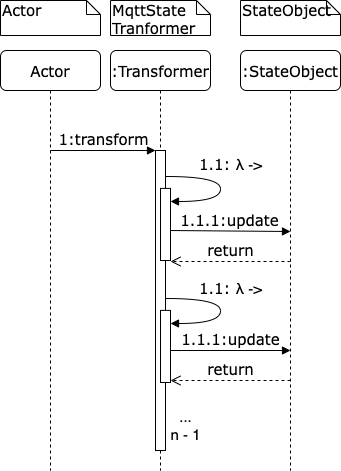
\includegraphics[width=14cm,height=8cm,keepaspectratio]{images/Transformation_old.png}
        \caption{Transformation über Switch-Case-Anweisung}
        \label{fig:sequenceTransformationOld}
    \end{figure}

\begin{lstlisting}[language=Java, frame=lines, xleftmargin=\parindent, style=algoBericht, label={code:switch-case}, captionpos=b, caption={Transformeation über eine Switch-Case-Anweisung}]
public class MqttTransformer extends AbstractTransformer<InnovationLabKA> {
    private final LogicHubState<InnovationLabKA> logicHubState;

    public void transform(String topic, String payload) {
        switch (topic) {
            case "InnovationLab/LogicHub/PersonOnDoor":
                logicHubState.setState((innovationLab) -> {
                    innovationLab.setPersonOnDoor(payload);
                    innovationLab.update();
                });
                break;
            case "InnovationLab/LogicHub/SR/GoTo":
                logicHubState.setState((innovationLab) -> {
                    innovationLab.setSRGoTo(payload);
                    innovationLab.update();
                });
                break;
        }    
    }
}
\end{lstlisting}
    Dieser Ansatz gibt eine Übersicht über die Topics und deren dafür vorgesehenen Zustandsänderungen. Nachteile dabei sind jedoch die Zunahme der Anweisungen, d.h. 
    je mehr Regeln und dafür vorgesehene Zustandsänderungen hinzugefügt werden, desto unübersichtlicher und länger wird die Switch-Case-Funktion, und die 
    Kenntnis der \acs{MQTT}-Topics an verschiedenen Stellen der Anwenderinteraktionen. Um innerhalb einer Regel eine weitere Zustandsänderung vornehmen zu können, muss der 
    Anwender das Topic erneut aufgreifen, damit über den \acs{MQTT}-Producer eine Nachricht veröffentlicht und eine Aktion ausgelöst wird. 
    \\
    Dieser unpraktische Lösungsweg galt es dem Anwender zu erleichtern, weshalb ein zweiter erarbeitet wurde, der im folgenden Abschnitt 
    aufgezeigt wird.

    \subsubsection*{Transformationsobjekt mittels eigenem Objekt}
        In Opposition zu der Verwendung einer Switch-Case-Anweisung wird bei diesem Ansatz eine Klasse implementiert, mit der je nach Bedarf 
        weitere Objekte mit unterschiedlichen Werten erzeugt werden können. Dabei werden in dem Konstrukt der Klasse die jeweiligen Parameter 
        definiert. Das zu erzeugende Objekt wird dem Framework zur Laufzeit übergeben und in einer Liste gespeichert, damit auf dieses zurückgegriffen werden kann. 
        Die Parameter, die der Entwickler bestimmt, haben folgende Funktion:
        \begin{itemize}
            \item 1. Parameter: Hier wird das Topic übergeben. Der \acs{MQTT}-Subscriber prüft, ob das konsumierte Topic einem in der Liste definierten entspricht.
            \item 2. Parameter: Hier wird der Key definiert. Das über das Topic mitgelieferte JSON-Konstrukt wird auf diesen Key überprüft. Dessen Wert ist für den Zustandsraum relevant. Hierüber wird der Zustand des Objektes transportiert.
            \item 3. Parameter: Hier wird optional eine Liste übergeben, die nur bestimmte Werte für den Key zulässt, eine sogenannte \textit{White-List}.
            \item 4. Parameter: Hier wird der Name des Feldes im Zustandsraum wiedergegeben, sodass mittels Reflection der Wert im Zustandsraum adressiert werden kann.
            \item 5. Parameter: Hier wird optional der Name des Komponentenfeldes im Zustandsraum wiedergegeben, sodass mittels Reflection der Komponentenwert im Zustandsraum adressiert werden kann.
        \end{itemize}
        Diese Werte bilden die Transformation, die ebenso für die Inverse (siehe Abschnitt \ref{subsec:inverseTransformation}) gilt.
        Der Ablauf kann dem folgenden Sequenzdiagramm entnommen werden: 
        \\
        \pagebreak
    \begin{figure}[hbt!]
        \centering
        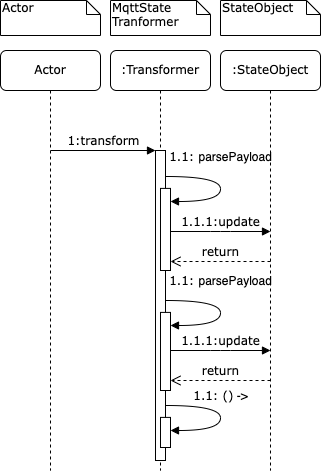
\includegraphics[width=14cm,height=9cm,keepaspectratio]{images/Transformation_new.drawio.png}
        \caption{Transformation über eigenes Objekt}
        \label{fig:sequenceTransformationNew}
    \end{figure}
    \\
    Um das Objekt zu erzeugen, muss der Entwickler lediglich das folgende Code-Beispiel verwenden und auf die entsprechenden Werte anpassen:
\begin{lstlisting}[language=Java, frame=lines, xleftmargin=\parindent, style=algoBericht, label={code:object}, captionpos=b, caption={Transformation über ein eigenes Objekt}]
public class InnovationLogicHubApplication {
    public InnovationLogicHubApplication() {
        ... 
        logicHub.addTransformation(
            new SimpleTopicTransformation(
                "InnovationLab/LogicHub/PersonOnDoor",
                "email",
                "personOnDoorEmail"
            )
        );
    }
}
\end{lstlisting}
    Für die jeweiligen Konfigurationsmöglichkeiten der Transformation existieren drei Konstrukte. 
    Neben der im Code-Beispiel (\ref{code:object}) aufgeführten gibt es die Struktur mit dem zusätzlichen Parameter der \textit{White-List}. 
    Die dritte Möglichkeit spiegelt zusätzlich den Namen eines Feldes innerhalb einer Komponente wieder. So können Objekte theoretisch in den Zustandsraum 
    aufgenommen werden, wovon allerdings zum aktuellen Zeitpunkt abgeraten wird. Die Begründung zu dieser Modellierung wird in dem Abschnitt 
    (\ref{subsec:modellierungsgrenzen}) aufgegriffen. 
    \\
    Der interne Ablauf des Frameworks unterscheidet sich bei beiden Transformationsmethoden in Nuancen, wie den beiden Sequenzdiagrammen 
    (\ref{fig:sequenceTransformationOld} und \ref{fig:sequenceTransformationNew}) zu entnehmen ist. Jedoch wird bei dem zweiten Ansatz 
    das Zustandsobjekt mittels Reflection manipuliert und anschließend als Änderung registriert und ausgeführt, während bei der ersten Methode 
    die Änderung direkt über die Lambda-Funktion gesteuert und ausgelöst wird. Dies hat für den Anwender keinerlei Auswirkung auf die 
    Funktionsweise des Frameworks. Innerhalb dieser Thesis war das Ziel die einfache Handhabung der formalisierten Interaktionen und 
    die übersichtliche Gestaltung. Der zweite Ansatz liefert dem Entwickler diese Vorteile und wird deshalb angewendet. 
    \\
    \linebreak
    Die Funktionsweise der Transformation ist demnach wie folgt umgesetzt:
    \\
    Die vorab definierten Transformationen des Entwicklers werden in einer Liste gespeichert, damit das darin enthaltene Topic mit dem vom \acs{MQTT}-Subscriber eingehenden 
    verglichen werden kann. Dafür wird die Liste wiederholt überprüft sowie jede Transformation und deren zugewiesenes Topic. Sofern 
    es eine Übereinstimmung gibt, wird der Key-Wert ermittelt und als Nutzlast (\textit{Payload}) übergeben. An dieser Stelle wird der \textit{ReentrantLock} aktiviert 
    und die Feldmanipulation für den Wert, der mittels Nutzlast mitgegeben wurde, durchgeführt. Nachdem die Zustandsänderung erfolgt ist, wird der \textit{Lock} deaktiviert und 
    die Zustandsänderung an die Logikschicht weitergegeben. Somit ist die Transformation für ein eingehendes \acs{MQTT}-Topic abgeschlossen. 
    Der Ablauf kann dem Sequenzdiagramm (siehe Abbildung \ref{fig:kommunikationsequenz}) entnommen werden.  
    \\
    Die Funktion der inversen Transformation wird im folgenden Abschnitt erläutert.

\subsection{Inverse Transformation}
\label{subsec:inverseTransformation}
    Damit der Anwender des Frameworks bei der Regeldefinition einen geringen Aufwand hat und dennoch dadurch eine weitere 
    Zustandsänderung hervorrufen kann, findet an dieser Stelle eine inverse Transformation statt. Dadurch wird anhand 
    der Zustandsänderung, die der Entwickler durch eine Funktion in der jeweiligen Regel vorgibt, die zugehörige Aktion mittels \acs{MQTT}-Nachricht 
    veröffentlicht. In Folge dessen muss der Entwickler bei der Implementierung einer Regel keine Kenntnis über das 
    \acs{MQTT}-Topic haben, lediglich muss das richtige Attribut im Zustandsraum angesprochen und geändert werden. 
    Ein konkretes Beispiel: 
    \\
    \linebreak
    Wird ein Lichtschalter betätigt, wird daraufhin ein \acs{MQTT}-Topic veröffentlicht und unmittelbar von der Steuerzentrale 
    konsumiert. Dadurch wird der Zustandsraum über eine Transformation geändert. Eine Regel, deren Regelaktion die LED-Leuchte aktiviert, wird ausgeführt. 
    Dementsprechend definiert der Entwickler eine Funktion, die den Wert des Lichtzustandes im Zustandsobjekt verändert. 
    Mit der Veränderung wird überprüft, um welches Attribut es sich im Zustandsraum handelt und wie sich der Wert geändert hat. 
    Wenn diese Bedingung zutrifft, wird im Rahmen der inversen Transformation ein \textit{JSON}-Konstrukt generiert, welches 
    mit dem in der Transformation definierten Topic als \acs{MQTT}-Nutzlast an den \acs{MQTT}-Broker publiziert wird. Dabei handelt 
    es sich konkret um das Topic, auf das der \acs{MQTT}-Client der LED-Leuchte reagiert.
    Daraufhin wird die LED-Leuchte angeschaltet. 
    \\
    \linebreak
    Zusammengefasst wird mit der inversen Transformation vermieden, dass der Entwickler sich bei der Regelimplementierung neben der zu definierenden 
    Zustandsänderung zusätzlich um das veröffentlichen der jeweiligen Nachricht und das Verpacken in eine übertragbare 
    \textit{JSON}-Struktur kümmern muss. Des weiteren ist die Kenntnis über das Topics, unter dem die Nachricht 
    gesendet wird, ausschließlich in der Transformation von Nöten und muss nicht an mehreren Stellen konkret 
    aufgeschrieben werden. Dafür kann zu jeder Zeit die Liste der Transformationen genutzt werden, um das erforderliche Topic zu erhalten. 
    \\
    \linebreak
    Zum aktuellen Zeitpunk wird bei der inversen Transformation ein einfaches \textit{JSON}-Konstrukt erzeugt. Dafür wird der 
    \textit{Key}-Wert der Transformation und die Nachricht als Nutzlast verwendet. Zur Veröffentlichung der Nachricht unter einem 
    \acs{MQTT}-Topic wird derzeit ausschließlich der \textit{Zigbee2MQTT}-Standard\footnote{Nutzung von Zigbee2MQTT. \url{https://www.zigbee2mqtt.io/guide/usage/mqtt_topics_and_messages.html} Besucht am 30.07.2022} 
    eingehalten. Dabei ergänzt sich die Topic-Zeichenkette, die über das Transformationsobjekt abgerufen werden kann, um den Anhang (\textit{/set}). 
    Hierfür wird vorab das \textit{JSON}-Konstrukt generiert, mit den jeweiligen Werten belegt und als Nutzlast mittels dem 
    Topic und dessen Anhang herausgegeben. Soll im Rahmen der Veröffentlichung einer Nachricht kein \textit{JSON}-Konstrukt sondern ein einzelner Wert 
    publiziert werden, so kann dies erfolgen, indem das Topic um den zugehörigen \textit{Key}-Wert der Transformation (\textit{/set/[Key-Wert]}) ergänzt wird. Ein Beispiel dazu:
    \\
    Eine LED-Leuchte wird mit einer Transformation mit den Werten (\textit{'mqtt/topic/test'}), \textit{'key-state'} und dem Attribut \textit{'led-leuchte'} 
    definiert. Soll in dem Zuge die Nutzlast nur den Wert \textit{'on'} enthalten, so wird kein 
    \textit{JSON}-Konstrukt erzeugt, sondern lediglich die Nachricht über das modifizierte Topic (\textit{'mqtt/topic/test/set/key-state'}) veröffentlicht. 
    \\
    \linebreak
    Resümierend gibt es im Kontext des \textit{Zigbee2MQTT} zwei Wege, um mit Geräten, die das ZigBee-Protokoll unterstützen, zu kommunizieren. Diese sind beide 
    über das Framework, somit auch über die inverse Transformation abgedeckt.

%
%Hierfür muss erneut eine  \acs{MQTT}-Nachricht 
%über ein bestimmtes Topic veröffentlicht werden. Diese Veröffentlichung findet im Rahmen der inversen Transformation statt Da diese Transformation bereits definiert wurde, ist innerhalb der Regel %ausschließlich die Zustandsänderung 
%zu definieren. Mithilfe der inversen Transformation wird anhand der Zustandsänderung die dementsprechende Aktion invertiert und unter 
%dem dafür vorgesehenen Topic eine Nachricht veröffentlicht, die die LED konsumiert und daraufhin das Licht angeschaltet. 

\subsection{Regeldefinition}
    Damit die Vorgaben für eine valide Regeldefinition eingehalten werden, wird dem Anwender mittels \textit{Template Methode}-Pattern 
    eine Schablone vorgeschrieben, die alle notwendigen Methoden bestimmt, die der Entwickler implementieren sollte. Zusätzlich gibt es eine Annotation, die 
    \textit{RuleAnnotation}, die eine Regel als solche kenntlich macht und die Implementierung der Methoden forciert. Die beiden wichtigsten Funktionen 
    innerhalb der Klasse, die durch die abstrakte Definition zum Softwareentwickler durchgereicht werden, sind zum einen die \textit{checkCondition}-Funktion und 
    zum anderen die \textit{ruleProcess}-Funktion. Innerhalb der erstgenannten Methode gibt der Anwender einen Sachverhalt vor, der zutreffen muss, sodass anschließend diese 
    Regel ausgeführt werden kann. Die Bedingung ist abhängig von dem Feld des Zustandsraumes und der Absicht, für die der Regelprozess gestartet werden soll. Sofern die 
    Bedingung zutrifft, wird ein boolescher Wert (\textit{true}) zurückgeliefert, der die Regel ausführen lässt. Die ebenso wichtige Funktion des Regelprozesses beinhaltet die Schritte der 
    Regelausführung als klassische Methode, die keinen konkreten Wert zurückgibt, sondern lediglich die darin enthaltenen Punkte abarbeitet. An dieser Stelle können wiederum 
    weitere Zustandsänderungen implementiert werden. Dies ist abhängig von dem Inhalt der Regel und liegt ebenso in der Verantwortung des Entwicklers. 
    \\
    Neben den beiden Hauptfunktionen gibt es eine weitere Funktion, die den Auslöser der Regel definiert. Diese dient dazu, um Regeln ggf. nur dann anstoßen zu können, wenn ein bestimmter 
    Auslöser dafür aktiviert wurde. Zusätzlich gibt es weitere Funktionen, die reine Informationswerte enthalten, wie den Regelnamen und die -beschreibung. Darüber hinaus gibt es für den 
    Entwickler keinerlei Einschränkungen das Regelobjekt um weitere Funktionen zu ergänzen. 

\subsection{Parallelisierung}
\label{subsec:parallelisierung}
    Bereits im Konzept wurde der Terminus der Parallelisierung und der Asynchronität aufgegriffen. Für das Auslösen einer Regel wird der gesamte Prozess der 
    Bedingungsprüfung und der anschließenden Ausführung in einen \textit{Thread} ausgelagert, der durch einen 
    \textit{ThreadPoolExecutor}\footnote{Spezifikation des Thread-Pools. \url{https://docs.oracle.com/javase/7/docs/api/java/util/concurrent/ThreadPoolExecutor.html} Besucht am 27.07.2022} im Java Code angestoßen wird. 
    Es können durch mehrere \textit{Threads}, die in sich asynchron arbeiten, mehrere Regeln gleichzeitig ausgeführt werden, sofern die Bedingungen dafür zutreffen. 
    \\
    Sowohl die parallele als auch die sequenzielle Ausführung können innerhalb der Regel Zustandsänderungen hervorrufen.
    \\
    Eine sequenzielle Ausführung der Regeln ohne Verwendung von \textit{Threads} wäre sehr ineffektiv und langsam, da eine Regel erst dann ausgeführt wird, wenn sie an der Reihe ist. Der Anwender weiß nicht, zu welchem 
    Zeitpunkt die gewünschte Aktion eintritt, da er die Anzahl der dazwischenliegenden Sequenzen nicht kennt. 
    Wenn bspw. ein Lichtschalter betätigt werden würde und davor noch zwei Regeln abgearbeitet werden müssten, würde dies Zeit in Anspruch nehmen, wodurch sich das Leuchten der Lampe verzögert. 
    \\
    \linebreak 
    In dieser Arbeit wird die parallele Ausführung bevorzugt. Jedoch ist es durch die Parallelisierung 
    notwendig, die innerhalb der \textit{Threads} eventuell entstehenden Zustandsänderungen anschließend 
    zusammenzuführen, indem der Wert auf das eigentliche Objekt übertragen wird. Trotz der hinzukommenden 
    Komplexität durch die Zusammenführung überwiegt der Vorteil, da 
    die gewünschte Aktion unmittelbar ausgeführt wird, unabhängig von den derzeit parallel laufenden Prozessen. 
    \\
    Damit die Zustandsänderung und die darauf zu erstellende Kopie entsprechend sauber durchgeführt wird, wird dieser gesamte Vorgang durch einen 
    Lock-Mechanismus, der durch einen \textit{ReentrantLock}\footnote{Spezifikation des Locks. \url{https://docs.oracle.com/javase/7/docs/api/java/util/concurrent/locks/ReentrantLock.html} Besucht am 27.07.2022} 
    realisiert ist, gesperrt. Dadurch ist sichergestellt, dass die Änderung sowie die Kopie für die weiteren Schritte tatsächlich zur Verfügung steht. 

\subsection{Regelwerk -und management}
    Anknüpfend an die abgeschlossene Transformation wird der Teil ausgeführt, der basierend auf der Zustandsänderung 
    alle bekannten Regeln überprüft und die zutreffenden abarbeitet. Wenn eine Zustandsänderung keiner konkreten Regel zugeordnet 
    werden kann, fehlt diese entweder, wurde davor schon ausgeführt oder der Entwickler beabsichtigt keine Ausführung und sie 
    wird ohne Auswirkung übertragen. 
    \\
    Damit jedoch voneinander unabhängige Regeln parallel ausgeführt werden können, wird der Prozess der Regelüberprüfung und -durchführung 
    in einen \textit{Thread} ausgelagert, wie bereits im Abschnitt der Parallelisierung (siehe \ref{subsec:parallelisierung}) beschrieben. Der Ablauf kann dem 
    Sequenzdiagramm (siehe Abbildung \ref{fig:logiksequenz}) ab dem Schritt \textit{1.5:copyState} entnommen werden. 
    \\
    \linebreak
    Nach Implementierung des Frameworks sind alle Grundlagen des Systems zur Umsetzung der Use Cases gelegt und kann auf seine Funktionalität getestet werden, um 
    Anhaltspunkte für die Evaluation (siehe Kapitel \ref{chap:evaluation}) zu schaffen. Der folgende Abschnitt behandelt die praktische 
    Umsetzung zweier Anwendungsfälle. 

\subsection{Implementierung von Anwendungsfällen}
    Zur Überprüfung des Frameworks wurden im Rahmen der Arbeit drei Anwendungsfälle implementiert, um anhand deren die Funktionsweise 
    darzustellen. Zum einen wurde die Steuerung einer LED-Lampe über einen Schalter und ein Steckdosen-Funkmodul umgesetzt, um einen Vergleich zwischen der 
    Regeldefinition in Home Assistant, \acs{OPENHAB} und der Steuerzentrale (InnovationLogicHub) ziehen zu können. Zum anderen wurden die beiden 
    Anwendungsfälle, die im Rahmen der Anforderungsanalyse (siehe Kapitel \ref{chap:anforderungsanalyse}) als Anwendungsfälle (\ref{sec:usecases}) definiert wurden, realisiert. 
    
    \subsubsection*{Lichtregelung}
    Der Lichtschalter-Anwendungsfall besteht darin, dass mittels einem physischen oder virtuellen Schalter eine LED-Leuchte eingeschaltet werden kann. Zur 
    Gegenüberstellung der Umsetzungen wurden jeweils die gleichen Komponenten im selben Netzwerk verwendet. Dadurch sind die identischen Voraussetzungen geschaffen. 
    Zu Beginn musste sichergestellt werden, dass die Komponenten mindestens das \textit{ZigBee}-Kommunikationsprotokoll unterstützen, damit über \textit{Zigbee2mqtt} 
    die Nutzung von \acs{MQTT} möglich ist. 
    \\
    Um eine Grundlage für die Analyse und Untersuchung der jeweiligen Plattformen zu legen, wurden im Rahmen dieser Arbeit zu Anfang bereits Instanzen von Home Assistant und 
    \acs{OPENHAB} gestartet. Diese wurden zur Umsetzung des einfachen Anwendungsfalls unter anschließender Beurteilung der Resultate genutzt. 
    Die Integration der Elemente in die jeweilige Plattform wird an dieser Stelle nicht weiter erläutert, zur Veranschaulichung wird 
    lediglich die Regeldefinition aufgegriffen. Im Fokus steht jedoch die Umsetzung über die Steuerzentrale.
    \\
    \linebreak
    Unter Anwendung des Frameworks werden im folgenden Abschnitt die Schritte dargestellt, die für die Realisierung des Anwendungsfalls notwendig sind: 
    \\
    Damit die Zustände der Komponenten abgebildet werden konnten, mussten diese im Zustandsraum hinterlegt werden. Da der Schalter sowie das Funkmodul 
    beide die Werte \textit{'on'} und \textit{'off'} über das Kommunikationsprotokoll versenden, wurde zur Abbildung der Zustandsattribute jeweils der \textit{String}-Datentyp gewählt. 
    Durch die Nutzung der \textit{lombok}-Bibliothek sind die \textit{Getter}- und \textit{Setter}-Methoden gegeben. 
    \\
    Anhand der definierten Zustandsattribute konnten anschließend die Transformationen für beide Komponenten implementiert werden. Dafür notwendig waren jeweils 
    die \acs{MQTT}-Topics, der Name des Wertes innerhalb des \textit{JSON}-Konstruktes, ggf. eine Liste der akzeptierten Zustandswerte und der Name des im Zustandsraum 
    definierten Feldes. Die Transformationen waren daraufhin dem Framework zu übergeben, damit diese in die dafür vorgesehene Liste aufgenommen und zur Laufzeit als Objekte 
    erzeugt werden konnten. Abschließend war die Regel zu definieren, darunter die zu prüfende Bedingung und die darauffolgende Aktion. Diese beinhaltet die Änderung des Zustandsattributes auf den Wert 
    des Schalters, worauf über die inverse Transformation die \acs{MQTT}-Nachricht publiziert wird, die an das Funkmodul gerichtet ist. 
    Die beiden Methoden sind überschaubar und mit einem Quellcode weniger als fünf Zeilen zu implementieren. Dem Ausschnitt (siehe Anhang \ref{code:switch}) 
    sind die Methoden zu entnehmen. 
    \\
    Die Umsetzung des Anwendungsfalls in Home Assistant stellte sich als umständlicher und aufwändiger dar. Hierbei ist im Kontext des Home Assistant 
    eine übergreifende Automation, zwei Szenen (Aktionen) für das Schalten des Lichts und ein Auslöser für jede Aktion des Schalters zu definieren. Die Konfigurationsdatei 
    erstreckt sich über 50 Zeilen, in denen die eigentliche Funktion eingefügt wird. Die Benutzeroberfläche gibt dem Anwender die Möglichkeit, anhand der Informationen die 
    Konfigurationsdatei zu erzeugen. Dadurch ist der Entwickler nicht an die \textit{YAML}-Struktur gebunden und kann ausschließlich die Werte, um die es sich handelt, eintragen. 
    Das Erstellen der Automatisierung über die Nutzeroberfläche erschließt sich dem Anwender von der Logik her einfacher, ist dennoch 
    aufwändiger durch viele Interaktionen. Ergänzend dazu ist dem Anhang ein Ausschnitt der Konfigurationsdatei beigefügt (siehe Anhang \ref{code:hoasAutomation}).
    \\
    \linebreak
    Ähnlicher Konfigurationsaufwand war bei der Umsetzung in \acs{OPENHAB} über die Benutzeroberfläche festzustellen. Das skriptbasierte Definieren von Regeln erfordert eine 
    längere Einarbeitungszeit, da die Semantik des \textit{ECMAScripts} oder die Funktionsweise von bspw. \textit{Blockly} erst erlernt und verstanden werden muss. Die Regeldefinition 
    mittels der \textit{Rule \acs{DSL}} hingegen kann mit der der Steuerzentrale verglichen werden. Diese ist in ähnlich wenigen Schritten realisiert. Der 
    Quellcode-Ausschnitt zeigt den Umfang der Regel über die \acs{OPENHAB} \acs{DSL} (siehe Anhang \ref{code:openhabSwitch}). 
    \\
    \linebreak
    Die folgenden Anwendungsfälle wurden ausschließlich über die Steuerzentrale umgesetzt. 

    \subsubsection*{Check-in mit einem Service-Roboter}
        Die Handlungsschritte, um einen Anwendungsfall mit dem Framework zu realisieren, gleichen sich grundlegend. 
        Damit alle für den Fall notwendigen Zustände abgedeckt sind, wurden diese in dem Zustandsraum hinterlegt. Zu den notwendigen Attributen 
        zählen unter anderem die E-Mail-Adresse, bzw. der Name der authentifizierten Person, die Verfügbarkeit des Service-Roboters, sowie dessen 
        ausführbare Prozesse. Anschließend wurden die Transformationen zur Erzeugung der Schnittstelle (siehe Kapitel \ref{subsec:transformation}) definiert. 
        \\
        \linebreak
        Sobald eine Person über die Kamera authentifiziert wurde, wird ein \acs{MQTT}-Topic gesendet, welches als Nutzlast ein \textit{JSON}-Konstrukt mit einem Zeitstempel, den 
        Vor- und Nachnamen, sowie die E-Mail-Adresse der Person übergibt. Anhand dessen wird im Zustandsraum der Wert der E-Mail geändert, woraufhin die Regeln auf ihre 
        Bedingung überprüft werden. Dabei wird die Regel zum Begrüßen und Einchecken des Gastes gestartet. Hierfür wird der Service-Roboter an die Tür geschickt, an der er den 
        Gast empfängt und begrüßt. Während der Roboter an die Tür fährt, checkt er die Buchungen und überprüft, ob die Person einen Platz gebucht hat. 
        Nachdem der Gast empfangen und eine Buchung gefunden wurde, checkt der Roboter die Person ein und gibt daraufhin Rückmeldung, dass die Person erfolgreich im 
        Büroplatzbuchungssystem eingecheckt wurde. Ist der Gast bereits angemeldet oder hat vorab keine Buchung getätigt, wird er aktuell darum gebeten, nachträglich 
        einen Platz zu buchen und darauf einzuchecken. 
        \\
        Die Regelabfolge kann zusätzlich dem Sequenzdiagramm (siehe Abbildung \ref{fig:sequenceRuleGreet}) entnommen werden.
        \begin{figure}[hbt!]
            \centering
            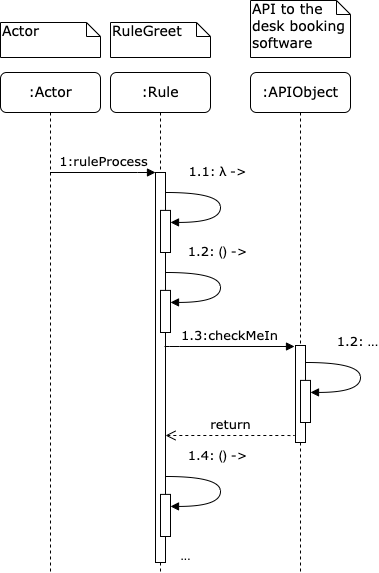
\includegraphics[width=14cm,height=12cm,keepaspectratio]{images/sequence_rule_temi_greet.png}
            \caption{Check-in Regelablauf (RuleProcess)}
            \label{fig:sequenceRuleGreet}
        \end{figure}
        \\
        %\pagebreak
        %\linebreak
        Der Check-in wurde im Rahmen dieser Arbeit als eine Handlungskette implementiert, da der Roboter zu aktuellem Zeitpunkt noch keine interaktiven Statusmeldungen geben kann. Dies 
        bedeutet, dass derzeit Befehle entgegengenommen werden können, darauf allerdings keine Rückmeldung erfolgt. Somit ist ein reeller Zustandsaustausch in Echtzeit nicht möglich. 
        Aus diesem Grund wurde nach jedem ausgehenden Befehl ein Intervall eingebaut, damit die Regel sequenziell abgearbeitet werden kann. Dafür wurden Zeitspannen definiert, die 
        der Roboter in etwa braucht, um einen Ortswechsel, bzw. einen Sprachbefehl durchzuführen. Eine alternative Lösung, sofern der Service-Roboter Statusmeldungen geben 
        könnte, wäre die feingranularere Aufteilung von einzelnen Prozessen, sodass erst nach erfolgreicher Rückmeldung des Roboters weitere Schritte eingeleitet werden würden.
        \\
        \linebreak
        Wird bspw. ein Sprachbefehl ausgeführt, so wird innerhalb der Regel über eine \textit{Lambda}-Funktion der Zustandsraum erneut geändert, wodurch die inverse Transformation 
        die Zustandsänderung überprüft und anhand deren der Sprachbefehl über ein \acs{MQTT}-Topic an den Broker gesendet wird. Hierbei reagiert der Roboter auf das Topic und führt 
        den Sprachbefehl aus. Diese Aktion ist dem Sequenzdiagramm (\ref{fig:sequenceRuleGreet}) unter anderem in den Schritten \textit{1.2:() ->} zu entnehmen. 
        \\
        Der Anwendungsfall wurde erfolgreich umgesetzt und konnte mit dem realen Service-Roboter getestet werden. 
        Ein \textit{Mock}\footnote{Simulierte Objekte in der Objekt-orientierten Programmierung. \url{https://en.wikipedia.org/wiki/Mock_object} Besucht am 02.08.2022} 
        des Service-Roboters wurde entwickelt, um die Interaktionen zu simulieren und die Usability-Tests durchzuführen. 
    
    \subsubsection*{Notfall-Evakuierung mit einem Service-Roboter}
        Der Anwendungsfall der Notfall-Evakuierung enthält ähnliche Handlungsschritte als die des Check-ins, weswegen dieser nicht detailliert 
        aufgegriffen wird. Die Prozessschritte sind ebenso möglich umzusetzen und wurden auch im Rahmen dieser 
        Arbeit realisiert. Der Ablauf ist in einigen Aktionen zu vergleichen mit dem im Sequenzdiagramm \ref{fig:sequenceRuleGreet} dargestellten. 
        \\
        Der Roboter selbst ist aktuell nicht in der Lage, Personen zu erkennen. Um dies zu vereinfachen, wurden im Rahmen dieser Arbeit 
        lediglich bestimmte Orte angefahren und die Warnmeldung ausgeführt. 
        
    \section{Fazit der prototypischen Implementierung}
        % Entscheidung für die Nutzung von Reflection. Begründung: Überprüfung der Werte im Zustandsraum, welche sich geändert haben. 
        %Und zur Nutzung der inversen Transformation, um an einer Stelle die Topics etc. zu definieren.
        Die Anwendungsfälle konnten wie erwartet umgesetzt werden und zeigen, dass die konzeptionellen Entscheidungen eine Grundlage für das 
        Framework darstellen. Die Regeln selbst können je nach Anwendungsfall beliebig definiert werden. An dieser Stelle werden dem 
        Entwickler alle Möglichkeiten ohne Einschränkungen offengelassen. Des weiteren ist der Schnitt zwischen 
        Anwender und Framework klar gegeben, indem der Softwareentwickler sich ausschließlich mit den Regeln, Transformationen und Zustandsattributen 
        befassen muss. Entscheidend ist die Gegebenheit eines \acs{MQTT}-Brokers, ohne diesen das Framework keine Verbindung aufbaut und kein Datentransfer, an dem 
        die Steuerzentrale teilnehmen kann, stattfindet. 
        \\
        \linebreak
        Mit der Konzeption der Transformation wird bereits zu Anfang ein zentraler Punkt gegeben, mit dem der Anwender alle notwendigen Informationen 
        bündeln und dem Frameworks zur Verfügung stellen kann. Anhand dieses Beschlusses kann der Entwickler die Zuordnung treffen, bspw. durch welches 
        eingehende \acs{MQTT}-Topic welches Attribut im Zustandsraum geändert werden soll. Mit der Entscheidung zur Nutzung der generischen Programmierung 
        und somit der flexiblen Gestaltung des Zustandsraumes musste überlegt werden, wie dieses Objekt dennoch zu überwachen und zu manipulieren ist. 
        Hierfür wurde die Java Reflection genutzt, die eine für diesen Fall geeignete Funktion der Java-Programmierung darstellt. Dennoch gibt es Hürden bei der Nutzung, 
        die im Rahmen der Konzeption hingenommen wurden, die allerdings zu keinen Einschränkungen führen. Trotz dessen kann durch die Einhaltung 
        der Modellierungsvorgaben (\ref{subsec:modellierungsgrenzen}) diese umgangen und so die Anwendungsfälle, die im Rahmen der Arbeit 
        definiert wurden, bzw. in der Umgebung eines smarten Büros auftreten können, umgesetzt werden. Entscheidend dabei ist die Definition der 
        Transformation sowie die der Regel selbst. 
        \\
        %\linebreak
        Der Prototyp erfüllt alle Voraussetzungen, um die definierten Anwendungsfälle umzusetzen.
    
    \subsection{Modellierungsvorgaben und -grenzen}
    \label{subsec:modellierungsgrenzen}
        Der Anwender muss für die Umsetzung jedes Anwendungsfalls folgende drei Punkte erneut implementieren: 
        \begin{enumerate}
            \item \textit{Das Attribut im Zustandsraum.}
            In der Klasse, in der die Zustandsattribute abgebildet werden, ist das Nutzen von einfachen Attributen, darunter 
            \textit{String}, \textit{Integer}, \textit{Double}, \textit{boolean} und \textit{Long}, empfohlen und vorgesehen. Es können 
            zwar Objekte hinzugefügt werden, diese werden jedoch nicht vom Framework berücksichtigt. 
            \\
            Theoretische wäre die Nutzung von Komponentenobjekten möglich und umsetzbar, jedoch werden im Kontext dieser Arbeit ausschließlich die einfachen Attribute verwendet. Was wiederum zur Folge hat, dass 
            durch die Nichtanwendung eine Grenze entsteht. Beim Versuch, den Zustandsraum um Objekte zu erweitern, wurde festgestellt, dass bei dem Kopiervorgang die Kopie eine neue Objektreferenz 
            auf dem Feld der Komponente erzeugt. Dies hat eine ungewollte simulierte Modifikation der Komponente zur Folge, die bei jeder Zustandsänderung hervorgerufen wird, ohne dass sie tatsächlich geändert wurde und 
            dadurch die inverse Transformation immer ausgeführt wird. 
            Dies ist ebenso keine absolute Grenze, die nicht umgangen werden könnte, lediglich durch den zeitlichen Faktor nicht weiter ausgeführt wurde. Für die Behebung müsste gegebenenfalls ein optimierter 
            Algorithmus zum Kopieren des Zustandsraums entwickelt, bzw. verwendet werden. 
            \\
            Da die Verwendung des Frameworks ausschließlich unter Gebrauch einfacher Attribute im Zustandsraum ohne weiteres funktioniert, wurde der Ansatz zur Nutzung von Komponenten vorerst verworfen.  
            % wiederum keine absolute Grenze, die nicht umgangen werden könnte, lediglich durch den zeitlichen Faktor nicht weiter ausgeführt wurde. 
            % Das Problem entsteht beim Verwenden von Objekten im Zustandsraum. 
            % Diese Tatsache ist den folgenden Punkten geschuldet: Bei einer Zustandsänderung muss über die Reflection eine absteigende Überprüfung des Komponentenobjektes innerhalb des Zustandsraums durchgeführt werden, um 
            % das adressierte Feld zu identifizieren. Dieser Vorgang ist eine Hürde, die jedoch noch umsetzbar wäre. Die eigentliche Grenze besteht Der wohl schwerwiegendere Punkt   innerhalb des Komponentenobjektes überprüft werden 
            
            % absteigenzum einen der Reflection geschuldet, da im Zustandsraum eine absteigende Überprüfung der einzelnen Felder 
            % innerhalb des Komponentenobjektes stattfinden muss, um Änderungen vernehmen zu können lediglich die Referenz des zur Laufzeit erzeugten Objektes 
            % steht, und zum anderen der Kopie des Zustandsobjektes, da innerhalb dieses Vorgangs eine neue Objektreferenz geschaffen wird, die als Änderung 
            % registriert wird. Das bedeutet jedoch nicht, dass immer eine Änderung des Objekts stattgefunden hat. 
            
            % Egal welches Attribut sich ändert, wird auf Grundlage dieser Änderung eine Kopie erstellt, die auf dem Objekt den Anschein erweckt, dass es sich geändert hat ohne tatsächlich geändert worden zu sein.  
            
            % bei dieser auf Grundlage der Kopie der daraus  hat, draus folgt dass bei der darauffolgenden Kopie ebenso der Anschein erweckt wird, dass sich das Objekt geändert hat ohne dass das explizit geändert wurde. 
            
            % Ebenso müsste sichergestellt 
            % werden können, um welches Attribut es sich innerhalb des Objekts handelt. Um dies zu garantieren, müsste das Hinzufügen von Komponenten ausschließlich im 
            % Zustandsraum zugelassen werden. Damit dies jedoch umgangen werden kann, wird vorerst die Nutzung von einfachen Attributen, darunter 
            % \textit{String}, \textit{Integer}, \textit{Double}, \textit{boolean} und \textit{Long} empfohlen. Andere Felder können zwar hinzugefügt werden, 
            % diese werden jedoch nicht vom Framework berücksichtigt.
            \item \textit{Die Transformation.}
            Die Transformation gibt ein klar definiertes Konstrukt vor. Dafür gibt es zwei Klassen, die implementiert werden können und 
            jeweils die Oberklasse \textit{AbstractTopicTransformation} erweitern. Zum einen ist dies die Transformation ohne 
            optionale \textit{White-List} von zugelassenen Werten und zum anderen diejenige, in der eine solche Liste übergeben werden kann. Über die 
            \textit{addTransformation}-Funktion wird zur Laufzeit das Transformationsobjekt erzeugt. Die Inhalte sind klar vorgegeben (siehe Abschnitt \ref{subsec:transformation}) 
            und müssen vom Entwickler entsprechend definiert werden.
            \pagebreak
            \item \textit{Die Definition der Regel.} 
            Die Definition einer Regel sieht vor, dass die Bedingung auf eine Zustandsänderung zutreffen muss. Der Regelprozess kann vom Anwender 
            frei implementiert werden. Zum Erstellen einer Regel ist zu Anfang zu garantieren, dass diese von der abstrakten Regelklasse erbt. So kann die Regel einer 
            Oberklasse zugeordnet und vom Framework als solche erkannt werden. Zusätzlich gibt es für die wichtigen Funktionen, die eine Regel zur 
            Implementierung bereitstellt, Annotationen. Sie geben syntaktische Metadaten vor, die das richtige Implementieren der Funktionen forciert. Die 
            Annotation muss beim Erstellen einer Klasse über der jeweiligen Funktion positioniert werden. Dem Quellcode-Ausschnitt im Anhang (siehe \ref{code:switch}) ist diese 
            syntaktische Hilfestellung zu entnehmen. Wichtig ist ebenso das Übergeben der definierten Regel an das Framework mittels der \textit{addRule}-Funktion. 
            \\
            Bei der Verwendung einer Bedingungsprüfung ist auf die Aussagekraft zu achten. Wird allerdings eine Bedingung so gewählt, dass sie bei jeder Zustandsänderung greift, kommt 
            es zu einer Rückkopplung und endlosen Ausführung. Dafür muss entweder innerhalb der Regel der Zustand wieder geändert oder eine treffendere Bedingung definiert werden.
        \end{enumerate}
        Diese Anmerkungen sind bei der Nutzung des Frameworks zu berücksichtigen, damit das Framework die Regeln und Prozesse entsprechend ausführt. 
    %WICHTIG: ZUSTANDSRAUM MODELLIERUNG VON KOMPONENTEN, BZW. OBJEKTE SIND MÖGLICH, 
    %Problematisch dabei ist die Prüfung der Zustandsänderung, da bei jeder Kopie eine neue 
    %Referenz der Komponente erzeugt wird, die eine Zustandsänderung unter dem Feld simuliert (vorgibt) ohne das diese tatsächlich stattgefunden hat.
    %UND DA DIE INVERSE TRANSFORMATION ZUM AUSLÖSEN VON AKTIONEN NUR DIE OBERSTE EBENE DES ZUSTANDSRAUMES ANSCHAUT UND ÜBERPRÜFT.
    % An dieser Stelle müsste feingranularer überprüft werden, dass allerdings nicht funktioniert. Heißt: aktuell werden nur die 
    %Änderungen auf der obersten Ebene überprüft das Absteigen in Objecte ist dabei nicht möglich, da das Object im Framework erst zur Laufzeit bekannt ist.
    
    % IST ABER AUCH NICHT NÖTIG, DA ALLE 
    %NOTWENDIGEN GEGENSTÄNDE ÜBER EINEN ODER MEHRERE ATTRIBUTE IM ZUSTANDSRAUM ABGEBILDET WERDEN KÖNNEN. BSP.? 
    % UND DIE ATTRIBUTE, BZW. DIE FELDER ÜBER DIE TRANSFORMATION GEBUNDEN WERDEN. 
    
    %Grenzen 
    %Modellierungsempfehlungen - Regel, Bedingung und Zustandraum 
    %Worauf man achten soll, wenn man ein neues Szenario abbildet. 
    %Modellierungsmöglichkeiten des Frameworks.
